\section{Идеи для хобби}
Хобби --- это способ уйти от скуки.
\begin{figure}[ht!]
    \centering
    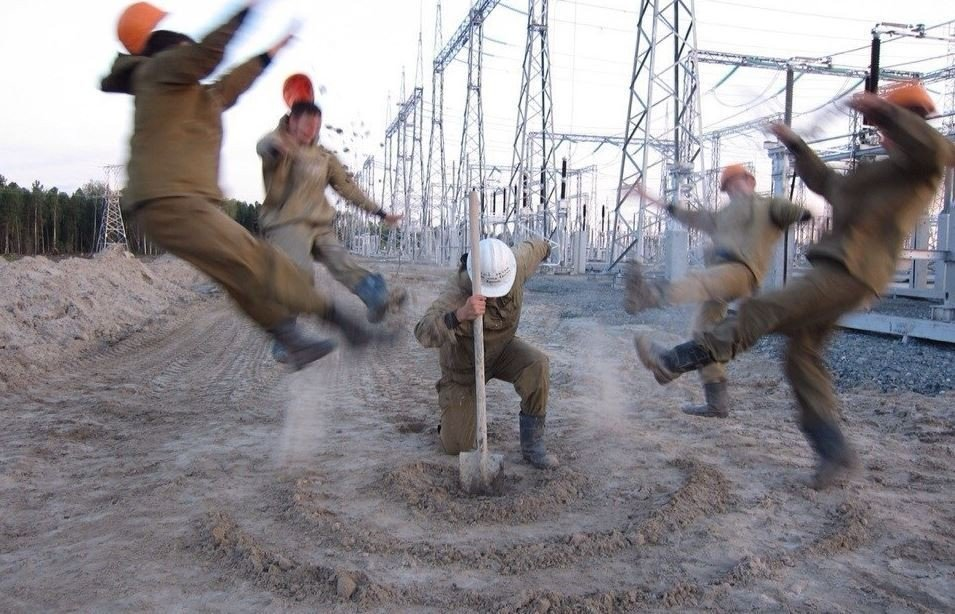
\includegraphics[width=\textwidth]{smile-please}
    \caption{not boredom, make photo}
\end{figure}
\begin{itemize}
\item Собирать идеи для хобби
\item Собрать библиотеку из самых странных (по содержанию, автору, оформлению и т.д.) книг из когда-либо выпущенных человечеством.
\item Искать забавные представления занятным числам:
  \begin{itemize}
    \item  $42 = 2^5 + 2 \cdot 5$
    \item  $145 = 1! + 4! + 5!$
    \item  $1729 = 19 \cdot 91 = 1^3 + 12^3 = 9^3 + 10^3$
    \item  $22 = 16_{16}$
  \end{itemize}
\item Придумывать скороговорки, начинающиеся/заканчивающиеся на одну букву:
\begin{flushleft}
\begin{verse}
Виолончелисты ввалились в вагон,\\
Виолончели выпали вкось.\\
Виолончелисты вышли вон,\\
Виолончели валяются врозь.\\

Виолончелисты в Вирджинии вдоль\\
Виолончели в ведро водрузили.\\
Виолончелисты внимательно вдаль\\
Виолончели вновь вукатили!\\

"Вертай всё взад" - вернувшись веолончедисты все вскричат.\\
Виолончель внутри вся влажная ---\\
Восвояси вскорь выпроважена.
\end{verse}
\end{flushleft}

\item (для ленивых) Коллекционировать прожитые годы.
\item Искать в других языках (и придумывать новые в своём) для обозначения различных странных состояний: как, например, называется состояние, когда есть желание вернуться в то место, из которого ещё не уехал?
\item Собирать/придумывать различные способы для изучения алфавитов.
% нужно переверстать данное место в TeX
\begin{figure}[ht!]
    \centering
    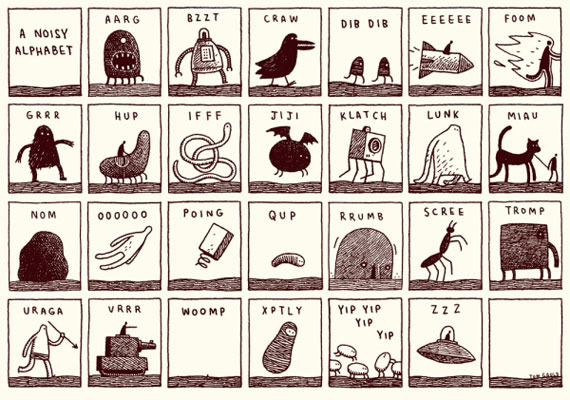
\includegraphics[width=\textwidth]{abc}
    \caption{Один из вариантов алфавита}
\end{figure}
\end{itemize}
